\documentclass[a4paper,11pt]{article}
\usepackage[utf8]{inputenc}
\usepackage{fullpage}
\usepackage{graphicx}
\usepackage{wrapfig}
\usepackage{caption}
\usepackage{subcaption}
\usepackage{appendix}
\usepackage{tcolorbox}
\tcbuselibrary{theorems}

\newtcbtheorem[number within=section]{theo}{}%
{colback=green!5,colframe=green!35!black,fonttitle=\bfseries}{th}

\title{% 
	Laser safety training \\
	\vspace{10pt}
	\small Summarized from L. Yales lecture, Michaelmas 2021}
\author{\small Oussama Chaib}
\date{\small October 2021}

\begin{document}
	\maketitle
	\begin{itemize}
		\item Must appy design and engineering controls (use enclosures).
		\item Risk assessment of experiment (justification of enclosure materials and eye/skin protection, justification of any open beams, beam hazard assessment).
		\item Must have local rules for your experiment/laser, if someone else's done one then it's ok. If the risk assessment is in your opinion incorrect or incomplete, then feel free to do one yourself.
		\item Procurement: must inform your LSO (laser safety officer) of any laser broughts/displaced.
		\item Must have evidence of appropriate trainings.
		\item Sometimes, visits are conducted by health and safety executive specialist radiation inspectors. The university could get into trouble if there's a breach.
		\item Risk assessment:
		\begin{itemize}
			\item Careful examination of what could harm people and whether your have enough precautions or should do more to prevent harm.
			\item Must make sure nobody gets ill (toxic fumes, migraine, geratin of Xrays), or hurt.
			\item There is a legal requirement to respect.
			\item Risks vs Hazards (the latter can cause risks).
			\item HSE 5 steps (identify hazards, decide who might be harmed and why (risk evaluation), write everything down in a risk assessment document, review and revise...)
		\end{itemize}
	\item Risks happen when we start to relax a bit after using the lasers/material for a while.
	\item Don't leave visitors alone with lasers.
	\item Laser application model, all are subject to risk assessment:
	\begin{itemize}
		\item Laser equipment: everything from the aperture backwards (power supply, cooling system, controls). Could be a mess (true) or neat.
		\item Beam delivery: from aperture to the point at which the laser beam is used (air, optical components, beam tubes, optical fibres). Must consider both normal use and alignment (stray beams, quality of optical mountings, alignment technique). Accident with someone who left his setup unaligned and didn't add any markers, someone walking from a lab to another caught a stray beams and got a peripheral vision damage.
		\item Laser process: absorption, reflection transmissions, optical hazard from reflected radiation, secondary hazards (glare, dazzle, distraction, fume, fire explosion).
		\item Environment and people: Back and forth (how they affect the laser and how they are affected by the laser).
	\end{itemize}
\item Some basics of laser radiation
	\begin{itemize}
		\item "Usually" monochromatic and unidirectional.
		\item High power densities.
		\item Damage possible even at a large distance from the source.
		\item High peak power at fraction of second for the case of pulsed lasers (peak power $\neq$ average power of your laser). The peak power does the bigger damage in this case.
	\end{itemize}
\item Biological hazards:
\begin{itemize}
	\item Potential eye damage. 
	\item Wavelengths: Retina captures visible + IR-A (interesting, also causes damage to the retina even if invisible), UV-A stopped at lens, UV-B, UV-C, IR-B, UR-C are stopped at the cornea but can damage it. (Why is UV split into many types? They have different properties, can penetrate up to X depth of skin).
	\begin{figure}[h]
		\centering
		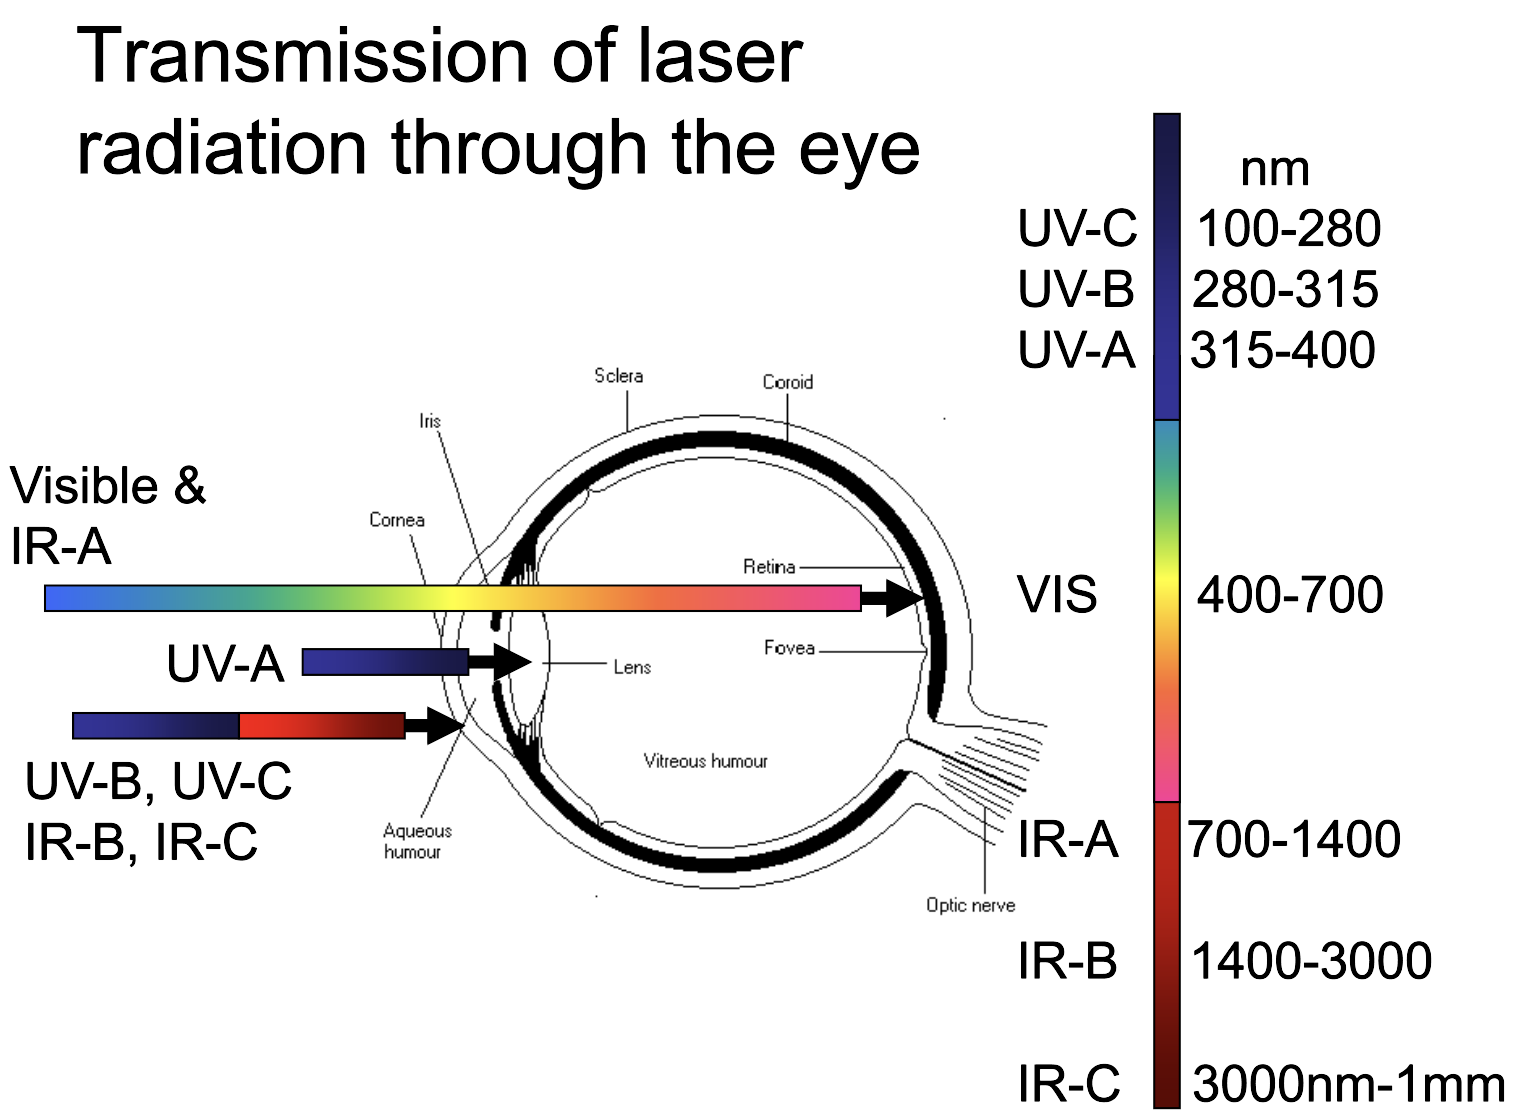
\includegraphics[width=.8\linewidth]{figures/eye.png}
	\end{figure}
\item Additive effects possible from different wavelengths.
\item Thermal effects, photochemical effects (dominate up to 550 nm, can arise from short high exposures or repeated low exposures = PIV wavelengths). Some damage: burns, catracts, UV is carcinogen...)
\item Acoustic effects (shock waves from short high energy pulses can cause physical damage to surrounding tissue).
	\begin{figure}[h]
	\centering
	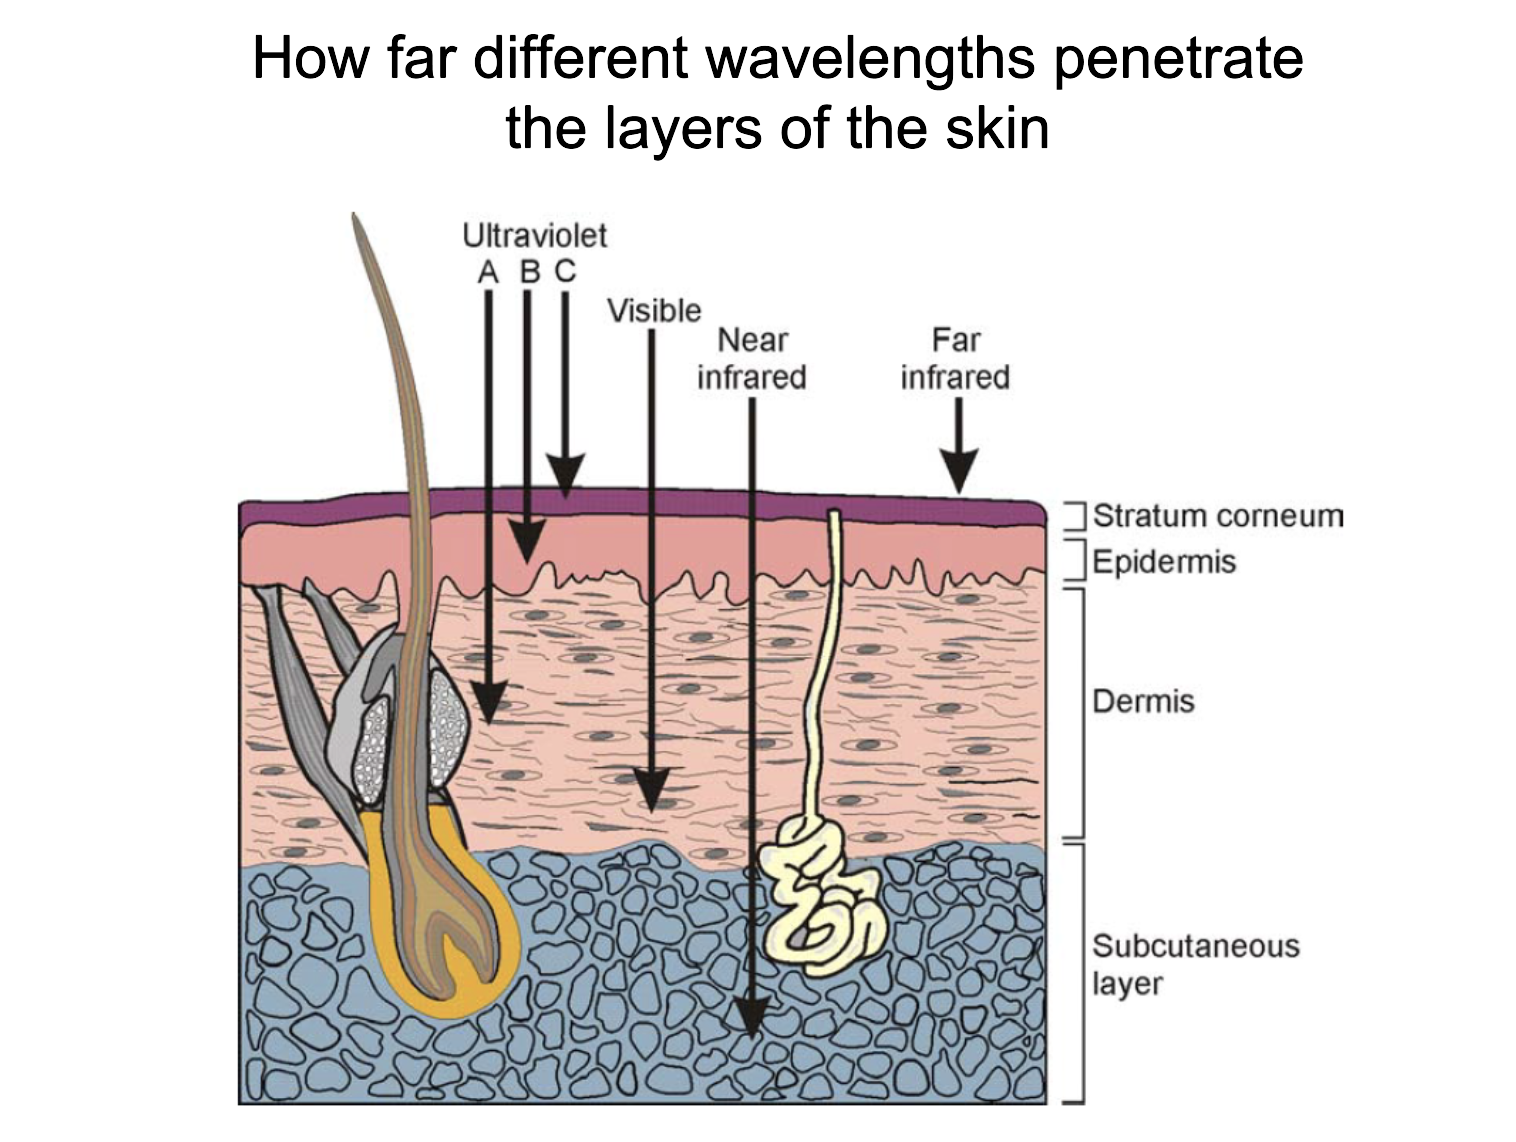
\includegraphics[width=.8\linewidth]{figures/skin.png}
\end{figure}
\end{itemize}
\item Different laser classes. Responsibility of manufacturer (warning labels). 
\item American classes are different than international classes.
\item Some metrics: AEL (accessible emission limit: maximum level of emission allowed for a certain class), MPE (maximum permissible exposure).
\item Laser classes: (M: magnifier, specular vs. diffuse a.k.a do we keep one beam or does it diffuse into different beams when reflecting on surfaces)
\begin{itemize}
	\item Class 1: $AEL<MPE$.
	\item Class 2: Safe to eyes if relying on aversion response (for a visible laser around .25 seconds). Safe to the skin. Only applies to visible lasers (1mW maximum).
	\item Class 3R: 5 times the MPE. Slight hazard to eyes. Safe to the skin. Cas de figure of accidents in Cambridge.
	\item Class 3B: Direct eye exposure not safe. Specular reflections are also not safe. Diffuse reflections safe if you don't look too close or for too long (viewing distance more than 13 cm, max viewing time 10 seconds).
	\item Class 4: Direct AND scattered radiation are damaging to both eyes and skin. Fire hazard associated too.
\end{itemize}
\item Laser beam hazard assessment: must consider any class 3B or 4 in use and any artificial source capable of presenting same level of hazard.
\begin{itemize}
	\item Must be done at a particular point in your system where things can go wrong.
	\item Assessment of the exposure can be ueful as part of your risk assessment.
	\item Combine with a plan of your laser setup.
	\item Questions: "Can I stick my head in the beam? What distance will I be able to? Any radiation effects?".
	\item Only need to do a laser beam assessment \textbf{at the point} in the setup where it could lead to hazards. Might want to put some warning signs but it's only really applicable where there is a reasonably unforseeable risk.
	\item Need to know: Power or energy/pulse, pulse duration, potential exposure duration, 
	\item Laser beam diameters: careful (green can seem bigger than red because of our eyes ). Defined by FWHM, beam diameter is 5\% of maximum. \\
	\textbf{Numerical apeture:} 1.7 x beam diameter at 1/e point.
	\item MPE: Irradiance or radiant exposure. Can be found on tables. Must be compared with worst case exposure at a specific location (eg at aperture). Do not use average power by default for pulsed lasers. To calculate irradiance or radiant exposure, we divide power or energy by an area, but what area? Depends on limiting aperture.
	\item If beam diameter greater than limiting aperture, divide by beam diameter, otherwise, average by limiting aperture.
	\item NOHD: Nominal ocular hazard distance (W/square meters), function of power, divergence (mrad), and diameter at aperture.	
	\item $C_6$: worse is when it's equal to 1 (MPE calculation?).
\end{itemize}
\item Associated hazards: 
\begin{itemize}
	\item Electrical hazards (high voltage, with perhaps cooling systems, risks if leakage or flooding, etc.) If electrical components are modified, we should consult another qualified person.
	\item Biological hazards.
	\item Chemical hazards.
	\item Mechanical hazards (gas cylinders, pressure regulators).
	\item Explosions (particles can be burnt).
\end{itemize}
\item Think about enclosures while building your system, do calculations to check if it's ok, get somebody else to check if it's okay.
\item Need local rules, risk assessment, safe working procedures. Have a look at "Safe rules for lasers".
\end{itemize}
\begin{figure}[h]
	\centering
	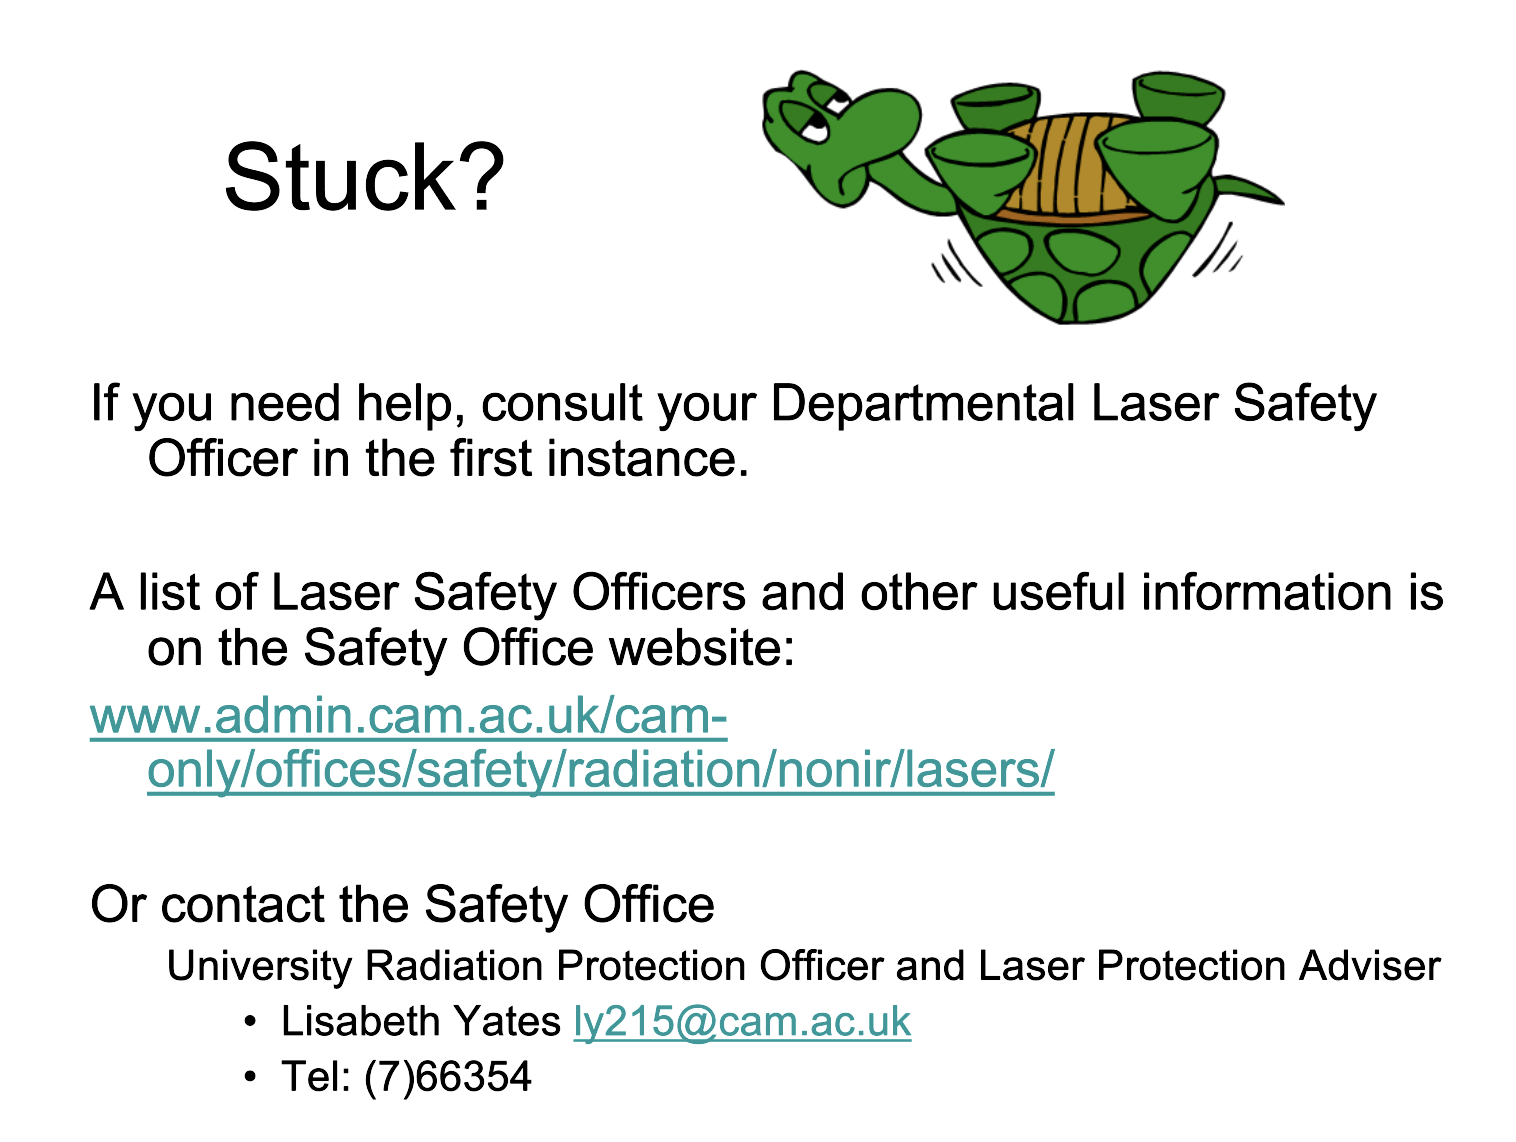
\includegraphics[width=.8\linewidth]{figures/contact.png}
\end{figure}
\end{document}






